\chapter{Font Features}




Using high-quality fonts is one goal.
This includes the fantastic \href{https://ctan.org/texarchive/fonts/tex-gyre/opentype}{\TeX Gyre fonts}, of which the \textit{Palatino} (by Hermann Zapf) clone \textit{Pagella} was chosen for this template.
It comes with an accompanying \href{https://ctan.org/texarchive/fonts/tex-gyre-math/opentype}{math font} of the same name.
As such, achieving a better match of text and maths fonts is nigh impossible.
Not only do the fonts look fantastic on their own, they (just as important) also feature an immensely broad support for symbols and characters, as well as font shapes and weights and combinations thereof.
The latter is demonstrated in \cref{tab:font_examples}.
%
\newcommand*{\sampletext}{The quick brown Fox jumps over the lazy Dog 13 times!}
\begin{table}
\ttabbox{%
	\caption[\TeX Gyre Pagella Examples]% Brackets hold entry that will go into List of Tables
	{%
		Examples for font features offered by \TeX Gyre Pagella%
	}%
	\label{tab:font_examples}% Use a string like 'tab:' to help with organization and auto-complete when reffing
}%
{%
	\begin{tabular}{@{}ll@{}}% Use @{} to remove white space from sides (since braces are empty)
		\toprule
			Feature & Sample Text\\
		\midrule
			Regular & \sampletext\\
			\textbf{Bold} & \textbf{\sampletext}\\
			\textit{Italics} & \textit{\sampletext}\\
			\textbf{\textit{Bold Italics}} & \textbf{\textit{\sampletext}}\\
		\addlinespace% Some ininconspicuous vertical separation; more visually pleasing than a full rule
			\textsc{Small Capitals} & \textsc{\sampletext}\\
			\textbf{\textsc{Bold SC}} & \textbf{\textsc{\sampletext}}\\
			\textit{\textsc{Italics SC}} & \textit{\textsc{\sampletext}}\\
		\bottomrule
	\end{tabular}
}%
\end{table}

Combine all that with \texttt{microtype}, and we have absolutely gorgeous typesetting.
As Jeremy Clarkson would say, \enquote{Behoooold the magnificence of this creation}:

\lipsum

\textbf{If you don't care for \textit{any} of this}, don't worry.
The features of \LaTeX{} and this template will do their work silently in the background.
%%%%%%%%%%%%%%%%%%%%%%%%%%%%%%%%%%%%%%%%%%%%%%%%%%%%%%%%%%%%%%%%%%%%%%%%%%%%%%%%%%%%%%%%%%%
\subsection{References}
Note that using the package \texttt{cleveref}, we only ever issue \verb|\cref| commands.
The package does the heavy lifting and puts the float type in front, also with correct plural forms if required.
Doing it any other way is just way too laborious.

The second most likely need for references are actual references for sources used in the work.
Examples are spread throughout this document.
At their basis, they rely on \texttt{biblatex} and its back-end \texttt{biber}.
Forget about \texttt{natbib} and similar tools.
Using \verb|\autocite{bibid}|, we can reliably cite sources and have a whole range of features delivered for free.
We do not have to worry about the specific citation style (in parentheses, as a superscript, \dots) --- \verb|\autocite{bibid}| takes care of that, we can then manage its behaviour globally.

Note the usage of --- in the previous sentence.
Use \verb|---| in the source code to have an em-dash---perhaps even without surrounding spaces?
That is probably up to your choice.
What is not, because it is largely agreed on, is to use \verb|--| -- an en-dash -- instead.
It is reserved for number ranges.
Lastly, a single hy-phen is reserved for just that --- hyphenation.
%%%%%%%%%%%%%%%%%%%%%%%%%%%%%%%%%%%%%%%%%%%%%%%%%%%%%%%%%%%%%%%%%%%%%%%%%%%%%%%%%%%%%%%%%%%
\subsection{Lists}
In technical publications, using lists (either bullet points or enumerations) is highly encouraged.
They should \textbf{always} be preferred over doing the same thing in a block of text.
Just consider this example list:
\begin{itemize}
	\item the presented approach is more complex than the previous one:
	\begin{enumerate}
		\item more time was spent doing computation,
		\item less time was spent effing about,
		\item features were added.
	\end{enumerate}
	\item at the same time, the following simplifications were made:
	\begin{enumerate}
		\item went from continuous- to discrete-time simulations,
		\item threw out some superfluous stuff.
	\end{enumerate}
\end{itemize}
Processing the very same information from a text paragraph is much less accessible.
Note the block-like \texttt{itemize} symbol, and the fact that enumerate numbers are part of the sans-serif family and bold.
This was specified and may be changed in the \texttt{enumitem} package options.
%%%%%%%%%%%%%%%%%%%%%%%%%%%%%%%%%%%%%%%%%%%%%%%%%%%%%%%%%%%%%%%%%%%%%%%%%%%%%%%%%%%%%%%%%%%
\subsection{Censoring}
Let me tell you a huge secret: \todo{I am a TODO note} \censor{today is \today}.
You can also censor float contents, as illustrated in \cref{fig:censorbox}.
\begin{figure}
	\ffigbox[\FBwidth]
	{%
		\caption{Example for a censoring box}%
		\label{fig:censorbox}%
	}%
	{%
		\censorbox{%
		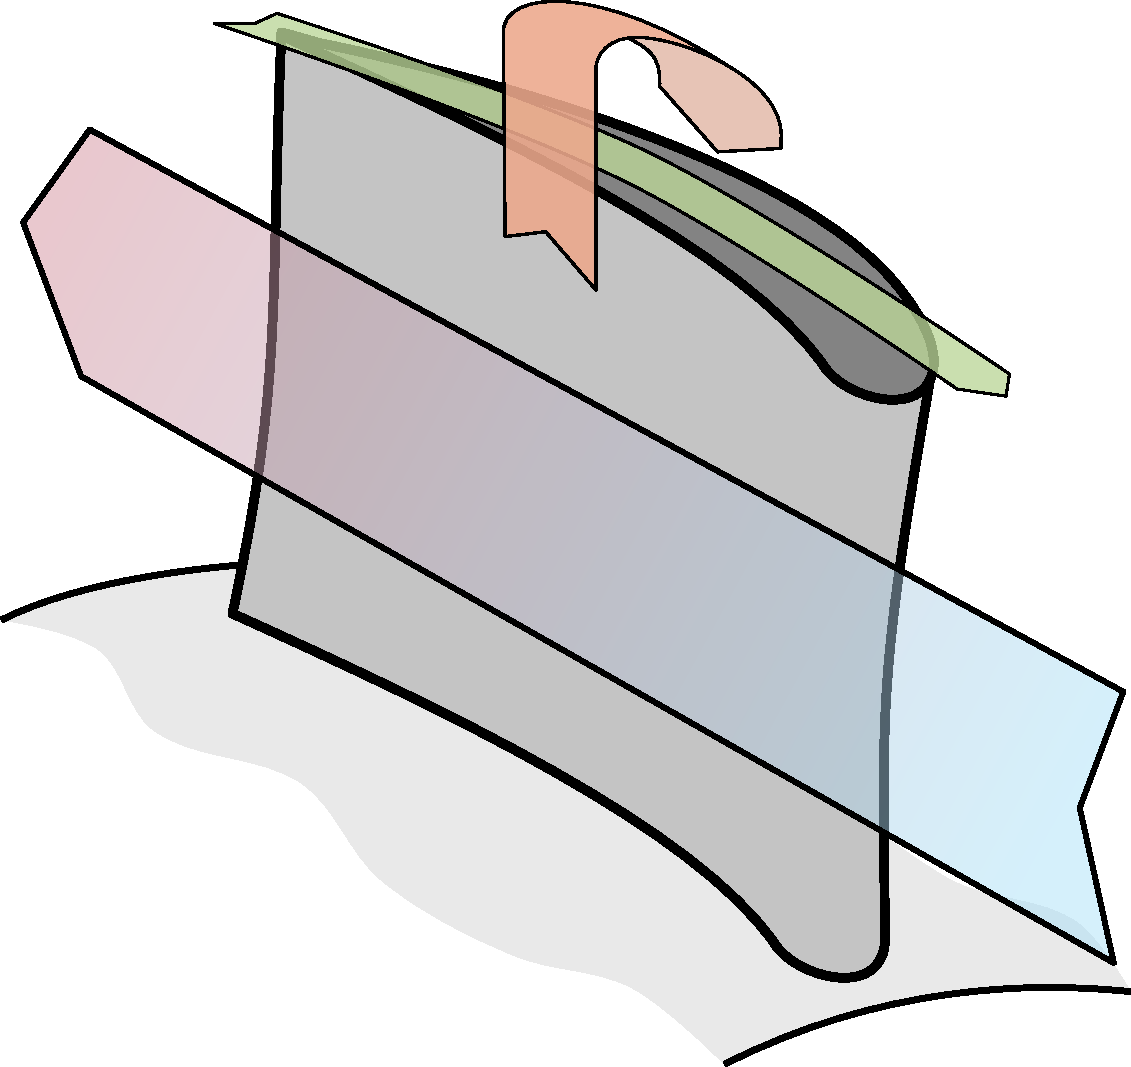
\includegraphics[width=0.5\textwidth]{example_image}% Having issued \graphicspath globally, we do not have to specify the full path here. Not even the file extension is strictly necessary.
		}%
	}
\end{figure}
%%%%%%%%%%%%%%%%%%%%%%%%%%%%%%%%%%%%%%%%%%%%%%%%%%%%%%%%%%%%%%%%%%%%%%%%%%%%%%%%%%%%%%%%%%%
%%%%%%%%%%%%%%%%%%%%%%%%%%%%%%%%%%%%%%%%%%%%%%%%%%%%%%%%%%%%%%%%%%%%%%%%%%%%%%%%%%%%%%%%%%%
